\documentclass[12pt]{article}
\usepackage[slovene]{babel}
\usepackage[utf8]{inputenc}
\usepackage[T2A]{fontenc}
\usepackage{amsmath}
\usepackage{amsfonts}
\usepackage{amssymb}
\usepackage[version=4]{mhchem}
\usepackage{stmaryrd}
\usepackage{graphicx}
\usepackage[export]{adjustbox}
\graphicspath{ {./images/} }
\usepackage{physics}
\usepackage{}
\usepackage{geometry}
\geometry{left=2cm,right=2cm,top=2cm,bottom=2cm}

\title{\textbf{Elektrooptični pojav}}
\author{Samo Krejan}
\date{marec 2025}

\begin{document}
\maketitle

\section{Uvod}

Z zunanjim električnim poljem lahko navadno vplivamo na strukturo snovi. V kristalih naprimer tako lahko spremenimo obliko osnovne celice, v tekočinah lahko pride do spremembe gostote in orientacijskega urejanja molekul ali pa celo do spreminjanja oblike posameznih molekul. Te spremembe seveda vplivajo tudi na optične lastnosti snovi. Mi se zanimamo za vpliv statičnih električnih polj na optične lastnosti snovi in temu rečemo \textit{elektrooptični pojav}. Če bi se zanimali za nestatična električna polja, bi bila to razprava \textit{nelinearne optike}.

Poznamo linearni elektrooptični pojav, ki se pojavi zgolj v anizotropnih snoveh, ter kvadratni elektrooptični pojav, ki ga lahko najdemo v vseh materialih. V splošnem, bi za opis elektrooptičnega pojava potrebovali tenzorje, a ker je naša keramika homogena in simetrična ob transformaciji $(x,y,z) \rightarrow (-x, -y,-z)$, zaradi česar se s tenzorji ne rabimo ukvarjati in je za to keramiko mogoč le kvadratni elektrooptični pojav. Zunanje elektroično polje zlomi simetrijo izotropne keramike, zato ločimo dve spremembi lomnega količnika: sprememba za svetlobo ki je polarizirana vzporedno z električnim poljem in za svetlobo, ki je nanj pravokotno polarizirana. 

V keramiko posvetimo z svetlobo z valovno dolžino $\lambda$ in variiramo zunanje električno polje jakosti $E$. Spreminjata se lomna količnika vzporedno $n_{\parallel}$ in pravokotno $n_{\perp}$ z smerjo polja. Oba se spreminjata s kvadratom električnega polja. Ponavadi nas ne zanima absolutna vrednost količnikov pač pa zgolj razlika med njima. To opisuje elektrooptični pojav poimenovan po Johnu Kerru \ref{Kerru}:

\begin{equation}
    n_{\parallel} - n_{\perp} = B\lambda E
    \label{Kerru}
\end{equation}
Konstanto $B$ imenujemo Kerrova konstanta. Elektrooptični pojav je osnova mnogih tehnologij, vse od atenuatorjev, do leč s spremenjivo goriščno razdaljo, tudi pri zapisovanju in branju optičnih informacij. 


\section{Potrebščine}

\begin{itemize}
    \item He-Ne plinski laser; $\lambda = 632.6\ nm$, vertikalno polariziran linearno,
    \item svetlobni modulator s PLZT keramiko, izvor visoke napetosti (0 - 1000V), voltmeter (multimeter),
    \item fotodioda vezana na namizni multimeter,
    \item polarizatorji pritrjeni na vrtljivih nosilcih,
    \item dvolomna celica iz tekočega kristala v nosilcu, ki omogoča vrtenje, kotomer,
    \item prenosnik z ustrezno programsko opremo.
\end{itemize}

\section{Naloga}
\begin{enumerate}
    \item Izmerite kotno odvisnost prepustnosti polarizatorja za linearno polarizirano svetlobo.
    \item Izmerite prepustnost dveh pravokotno postavljenih polarizatorjev, ko med njiju postavite tretji polarizator in ga vrtite.
    \item Določite Kerrovo konstanto PLZT keramike.
    \item Analizirajte polarizacijo svetlobe po prehodu skozi dvolomno snov in določite debelino celice.
\end{enumerate}


\section{Rezultati in analiza}


Pri prvem delu naloge pričakujemo zvezo med zasukom polarizatorja in prepuščeno močjo svetlobe kot \ref{poli1}

\begin{equation}
    P(\phi) = P_0 + P_1\ \sin^2 \left(\phi + \delta\right)
    \label{poli1}
\end{equation}
To funkcijo smo fittali na izmerjene podatke, s čimer smo dobili vrednosti parametrov:
\begin{equation*}
    P_0 = (1.8 \pm 0.8) 10^{-6} A,\ P_1 = (1.13 \pm 0.01) 10^{-4} A,\ \delta = -4.59 \pm 0.06
\end{equation*}
Uspešnost fita lahko opazujemo na grafu \ref{1poli}:

\begin{figure}[ht]
\begin{center}
    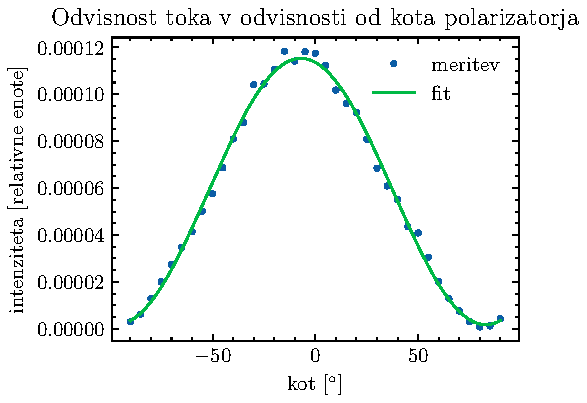
\includegraphics[width=10cm]{poli1.pdf}
    \caption{Meritve in fit meritev glede na enačbo \ref{poli1}}
    \label{1poli}
\end{center}
\end{figure}

Podobno situacijo opazujemo, ko med dva ortogonalno postavljena polarizatorja postavimo tretjega in ga vrtimo. Tam pričakujemo zvezo \ref{poli2}:

\begin{equation}
    P(\phi) = P_0 + P_1 \sin ^2 \left(2\phi + \delta\right)
    \label{poli2}
\end{equation}
Tu z fitom na izmerjene podatke dobimo vrednosti:

\begin{equation*}
    P_0 = (2.1 \pm 0.4) 10^{-6} A,\ P_1 = (2.05\pm 0.06) 10^{-5} A, \ \delta = 1.57 \pm 0.02
\end{equation*}
Spet uspešnost fita prikažemo na grafu. Glej graf \ref{2poli}:

\begin{figure}[ht]
\begin{center}
    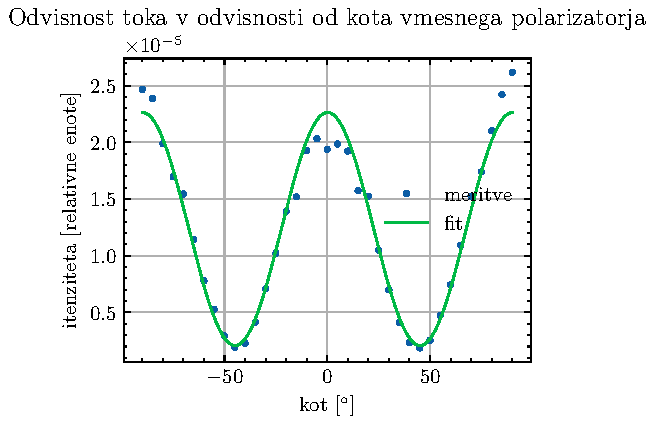
\includegraphics[width=10cm]{poli2.pdf}
    \caption{Meritve in fit meritev glede na enačbo \ref{poli2}}
    \label{2poli}
\end{center}
\end{figure}

S tem smo zaključili s prvim in drugim delom naloge. Sledila je meritev kerrove konstante za PLZT keramiko. Merili smo moč na fotodiodi v odvisnosti od napetosti na Kerrovi celici. V teoriji naj bi bili te dve količini povezani preko relacije \ref{fit1}:
\begin{equation}
    P(U) = P_0 \sin^2\left(\pi B L U^2/d^2 + \delta/2\right)
    \label{fit1}
\end{equation}
A kot lahko vidimo na grafu \ref{kerr}, ta fit ni najboljši, a ga lahko popravimo tako, da upoštevamo nek efektiven padec napetosti pred Kerrovo celico. Torej relacijo bolje opiše \ref{fit2}:
\begin{equation}
    P(U) = P_0 \sin^2\left(\pi B L (U-U_0)^2/d^2 + \delta/2\right)
    \label{fit2}
\end{equation}

\noindent Oba fita in meritve prikažemo na grafu \ref{kerr}, kjer se super vidi kako bolj uspešen je drugi fit \ref{fit2}.

\begin{figure}[ht]
\begin{center}
    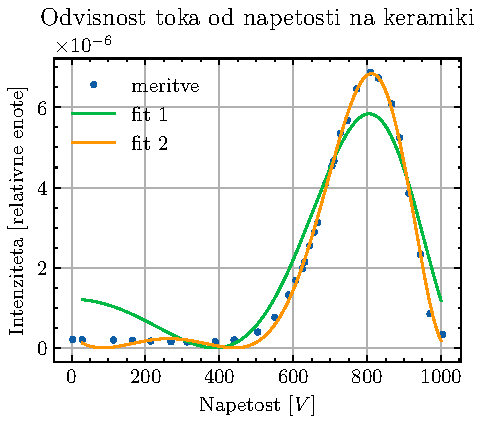
\includegraphics[width=10cm]{kerr.pdf}
    \caption{Fit 1 ustreza enačbi \ref{fit1}, fit 2 pa enačbi \ref{fit2}. Na grafu vidimo tudi meritve}
    \label{kerr}
\end{center}
\end{figure}

\noindent Iz drugega fita lahko izluščimo tudi parametre:

\begin{equation*}
    P_0 = (8.84\pm 0.06) 10^{-6} A,\ \frac{\pi B L}{d^2} = (5.8\pm 0.1) 10^{-6}V^{-2},\ \delta = -0.37\pm 0.03,\ U_0 = (263\pm 6) V
\end{equation*}

\newpage
\noindent Iz tega lahko izrazimo Kerrovo konstanto kot:

\begin{equation*}
    B = (2.27\pm 0.04) \cdot 10^{-9}\ m V^{-2}
\end{equation*}

\noindent V nadaljevanju smo Kerrovo celico zamenjali s tekočim kristalom. Od te točke naprej sam nisem imel preveč sreče z meritvami zato sem obdeloval podatke prijatelja Ruja, ki je svoje prijazno delil z menoj.

Najprej smo merili eliptično polariziranost tekočega kristala, ki nastane zaradi dvolomnosti tekočega kristala. Na meritve smo fitali relacijo \ref{tk-poli} in nato fit skupaj z meritvami prikazali na grafu \ref{tkpoli}:

\begin{equation}
    P(\phi) = P_0 + P_1\ \sin^2 \left(\phi + \delta\right)
    \label{tk-poli}
\end{equation}

\begin{figure}[ht]
\begin{center}
    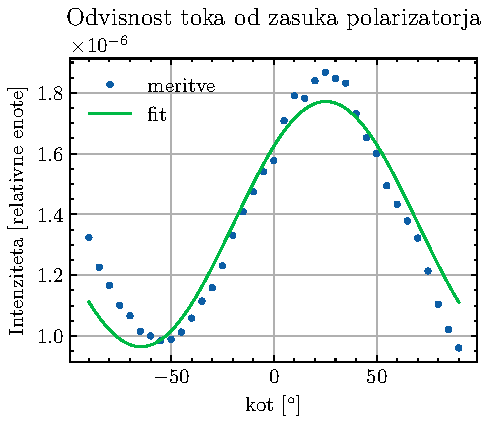
\includegraphics[width=10cm]{tkpoli.pdf}
    \caption{meritve in fit po enačbi \ref{tk-poli}}
    \label{tkpoli}
\end{center}
\end{figure}
O veljavnosti fita glede na graf bi se dalo mnogo diskutirati, a zaenkrat naj le povemo o parametrih, ki smo jih s pythonom izmerili:

\begin{equation*}
    P_0 = (1.77\pm 0.03)10^{-6}A,\ P_1 = (-8.1\pm 0.4)10^{-7}A,\ \delta = -0.44\pm 0.03
\end{equation*}

\noindent Torej imata lastni osi smer $-25.2^{\circ}$ in $64.8^{\circ}$. Prav tako lahko določimo ekscentričnost eliptičnosti polarizacije kot:

\begin{equation*}
    \epsilon = \sqrt{1-\frac{P_0^2}{(P_0 + P_1)^2}} = 0.73 \pm 0.01
\end{equation*}
čeprav, glede na uspešnost fita, se na te številke ne bi preveč naslajal.

\newpage
\noindent V zadnjem delu naloge je ostalo še izmeriti debelino ploščice tekočega kristala, tako da smo opazovali kaj se dogaja z intenziteto, ko vrtimo tekoči kristal okoli navpične osi. V teoriji bi morala prepuščena moč slediti enačbi \ref{last}:

\begin{equation}
    P(\phi) = P_0 + P_1 \sin^2\left(\frac{\pi d}{\lambda}(\sqrt{n_{\perp}^2 - \sin^2 \phi} - \sqrt{n_{\parallel}^2 - \sin^2\phi})\right)
    \label{last}
\end{equation}

S to enačbo fitamo izmerjene podatke, ki jih skupaj s fitom prikažemo na grafu \ref{balet}.

\begin{figure}[ht]
\begin{center}
    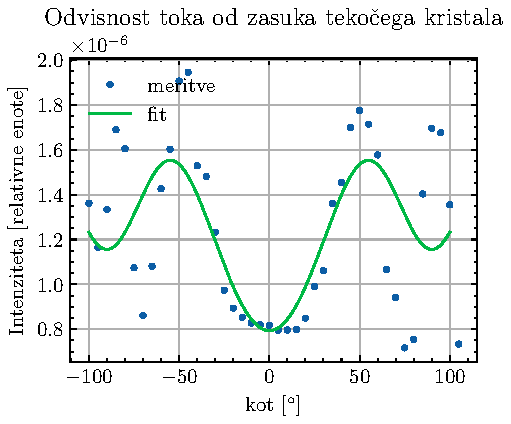
\includegraphics[width=10cm]{tk-balerina.pdf}
    \caption{Meritve in fit po enačbi \ref{last}}
    \label{balet}
\end{center}
\end{figure}
Tudi tukaj hitro vidimo, da je fit precej uprašljiv, ampak vsaj v osrednjem območju deluje kar zanesljivo. Iz omenjenega fita izluščimo parametre:

\begin{equation*}
    P_0 = (1.55\pm 0.08)10^{-6} A,\ (-4 \pm 1) A, \ \frac{\pi d}{\lambda} = 15.6\pm 0.1
\end{equation*}
iz česar sledi da je debelina ploščice tekočega kristala:

\begin{equation*}
    d = (3.18\pm 0.02) \mu m
\end{equation*}



\end{document}